\chapter{Overall Concept of the Developed Solutions}

\todo{Add chapter introduction}

% In this first result chapter of the thesis the overall concept which clarifies the relationship of the investigated issues is introduced.
% From this overall concept all further result chapters and the solutions covered by each of these chapters should be derived.

\section{BestRentalPoC}

The BestRentalPoC is a proof of concept for the usage of decentralized identities.
BestRental is a fictive car rental company, which requires customers to have a valid driver's license
when renting a car.
For this purpose, the driving license authority can issue a customer, called Alice, a verifiable credential (VC).
The VC is stored in Alice's digital wallet.
When renting a car, Alice can present her VC to BestRental, who can then verify the validity of Alice's driver's license.

The BestRentalPoC consists of three parts: The BestRental application, the DrivingLicenseAuthority application
and the decentralized identity system.
The BestRental application allows Alice to rent a car and present her VC.
The DrivingLicenseAuthority application allows the issuance of a VC to Alice.
Finally, the decentralized identity system provides the functionality of issuing and verifying VCs.

The BestRental application consists of a browser-based frontend and a microservice, which handles the required
business logic. In the same way, the DrivingLicenseAuthority application consists of a frontend and a microservice.
Additionally, both applications have tenants in Microsoft Azure which include an Azure Active Directory and
a Key Vault called VerifiedIDVault.

The decentralized identity system consists of Microsoft Entra Verified ID and the Trust System called DidWeb.
This proof of concept utilizes Microsoft Entra Verified ID to implement decentralized identities.
Entra provides all services which are required for this. This includes services to issues and to verify VCs.

Figure \ref{fig:sps_architecture_bestrental} shows the SystemPlusSoftware Architecture of the Demonstrator BestRental.

\begin{figure}
	\centering
	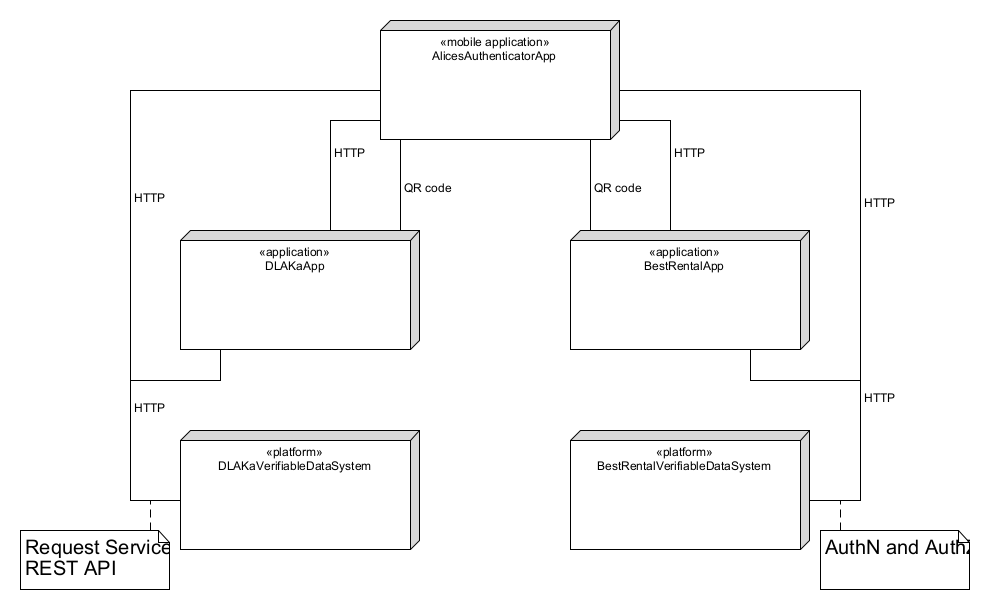
\includegraphics[width=\textwidth]{figures/sps_BestRentalPOC.png}
	\caption{SystemPlusSoftware Architecture BestRental}
	\label{fig:sps_architecture_bestrental}
\end{figure}